% The document class marks this as a poster, supplying various options that
% control rendering of some standard features (e.g., the title bar).

\documentclass[ % the name of the author
                    author={Luke Murray},
                % the name of the supervisor (preferably including title)
                supervisor={Dr. Simon Hollis},
                % the thesis    title (which cannot be blank)
                     title={Shadow Peer-to-Peer Networks},
                % the thesis subtitle (which can    be blank)
                  subtitle={},
                % the degree programme (from BSc, MEng, MSci, MSc and PhD)
                    degree={MEng},
                % the year of submission
                      year={2013} ]{poster}

\usepackage{epstopdf}
\usepackage{algorithm2e}
\begin{document}

% -----------------------------------------------------------------------------

\begin{frame}{} 

\vfill

\begin{columns}[t]
    \begin{column}{0.900\linewidth}
    \begin{block}{\normalsize Introduction}
    \small Shadow P2P is a network designed to provide a level of anonymity that has never been provided before. In existing networks, it is very hard to tell who is talking with who and what they are talking about. In additon to these features, my network aims to prevent anyone from being able to tell if a person is participating in the network or not. This is a feature not offered by any other network. This is achieved through the use of several key project components. Among these are: shouts, shout groups, public key hiding and a toroidal network structure.
    \end{block}
    \end{column}
\end{columns}

\vfill

\begin{columns}[t]
    \begin{column}{0.422\linewidth}
    \begin{block}{\normalsize 1. Shouts}
    \small A shout is how peers communicate anonymously. To do this, the sender gets the shout list corresponding to the receiver.
    \begin{figure}[h]
        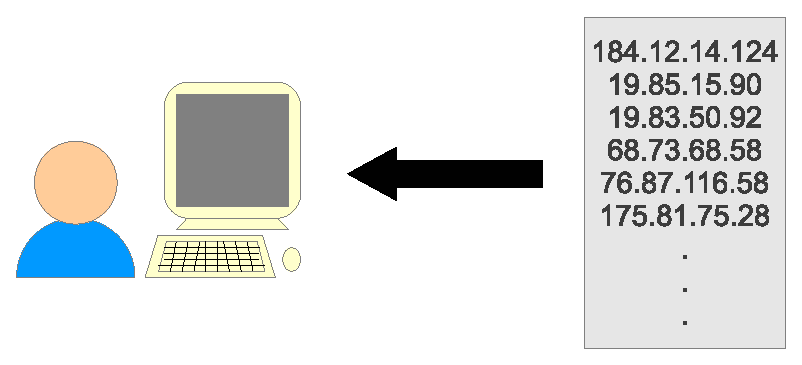
\includegraphics{diagrams/poster_get_list.eps}
    \end{figure}
    The sender then sends messages to the receiver by sending packets with a spoofed source IP address to every IP address in the shout list.
    \begin{figure}[h]
        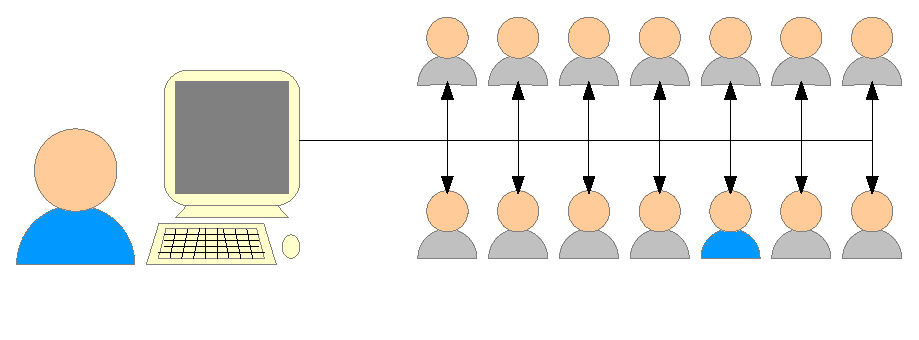
\includegraphics{diagrams/poster_d2.eps}
    \end{figure}
    This method of communication is unreliable and very inefficient but it does remove most of the information about the peers' identities. The point of most concern is that some party could search through the IP addresses in the shout list to find the true identity of the peer. For that reason, shout groups have been created.
    \end{block}
    \end{column}

    \begin{column}{0.422\linewidth}
    \begin{block}{\normalsize 2. Shout Groups}
    \small Shout groups are a defence mechanism that prevents adversaries from searching through the IP addresses in the shout list. A small number of peers work together and create a joint shout list that contains all of their real IP addresses.
    \begin{figure}[h]
        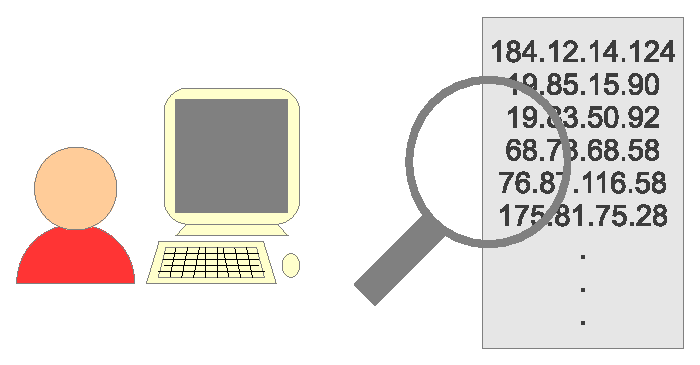
\includegraphics{diagrams/poster_search_list.eps}
    \end{figure}
    These peers work together to ensure that they only respond to messages that do not give their identities away.
    \begin{figure}[h]
        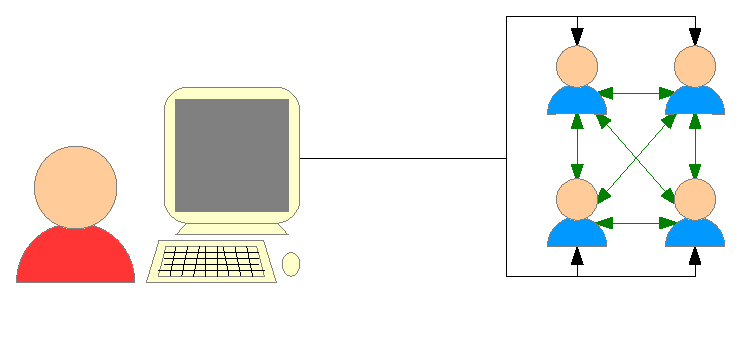
\includegraphics{diagrams/poster_d3.eps}
    \end{figure}
    The aim of the shout group is to minimise the amount of information that a hostile sender can gain about the peers' IP addresses. Here, we also need to consider the cases where members of the shout group are hostile and how we reduce the frequency of these attacks.
    \end{block}
    \end{column}
\end{columns}

\vfill

\begin{columns}[t]
    \begin{column}{0.422\linewidth}
    \begin{block}{\normalsize 3. Public Key Hiding}
    \small Peers are associated with a public key. This can reveal who is communicating with whom, even with anonymous identities. To prevent this I have invented a method of hiding a public key such that it becomes unrecognisable but so that it can still be used for encryption. In ElGamal, this can be done as follows:
    \begin{figure}[h]
        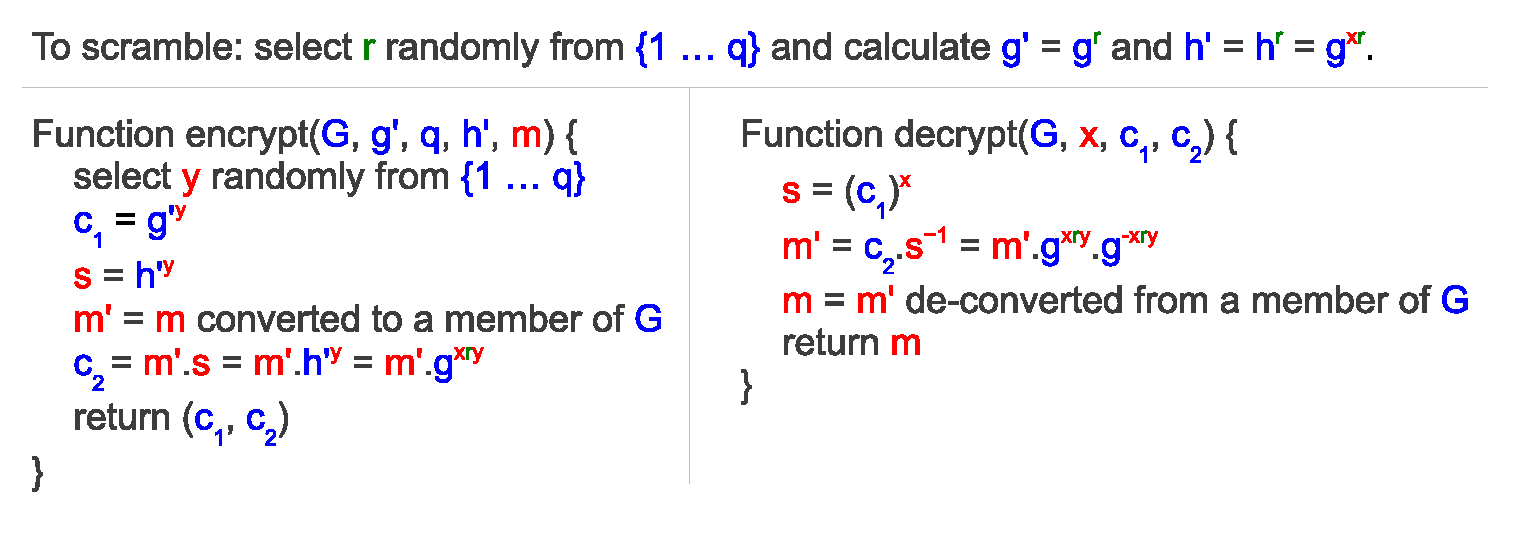
\includegraphics{diagrams/poster_d4.eps}
    \end{figure}    
    This method of public key hiding also works with ECIES (Elliptic Curve Integrated Encryption Scheme).
    \end{block}
    \end{column}
    
    \begin{column}{0.422\linewidth}
    \begin{block}{\normalsize 4. Network Structure}
    \small The network uses a uni-directional toroidal structure through which to deliver packets. This regular structure allows packets to be routed in many different ways making it very difficult to perform traffic analysis. The structure also allows easy dynamic expansion and contraction of the network.
    \begin{figure}[h]
        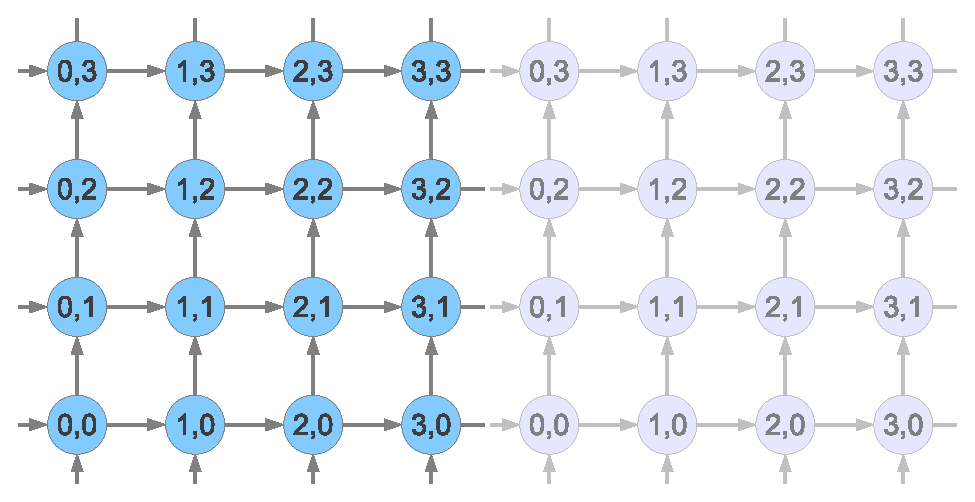
\includegraphics{diagrams/poster_d1.eps}
    \end{figure}
    Nodes transform packets that pass through them so that packets cannot be traced. By using source routing, the sender can be assured that their packets are routed randomly.
    \end{block}
    \end{column}
\end{columns}

\vfill

\end{frame}

% -----------------------------------------------------------------------------

\end{document}



